\section{Sistemi za kontrolu verzija}

Pisanje koda je proces koji se odvija u više iteracija. Naime, kada se kod piše, neretko se dešava da dolazi do ozbiljnih strukturnih promena i izmena u kodu, ili nekih dopuna koje zahtevaju novu verziju koda. Najčešće, ono za čime se prvo poseže, kako bi se nova verzija odvojila od stare, jeste  kreiranje novih foldera, kojih posle nekog vremena može biti previše čime se dodatno otežava rad i prate promene koda. Ovakav pristup je veoma podložan greškama i može napraviti ozbiljne probleme.
Sistemi za kontrolu verzija (engl. Version Control Systems) predstavljaju neizostavan deo procesa razvoja softvera. Oni spadaju među neophodne alate prilikom kreiranja softvera i pomažu programerima da isprate, često, veoma brojne promene u kodu, strukturi dokumenata, kao i da zajednički rade nad istim fajlovima. Zahvaljujući njima nema potrebe za ručnim prebacivanjem fajlova sa računara na računar, beskrajnim objašnjavanjima koje su promene izvršene i sličnih problema koji bi oduzeli nesrazmerno mnogo vremena.\\\\
Postoje mnogobrojne prednosti korišćenja sistema za kontrolu verzija, neke od glavnih su to što omogućavaju korisnicima da prate promene prilikom razvoja softvera, dozvoljavaju im da sarađuju na razvoju koda, omogućavaju pregled istorije razvoja koda, vraćanje koda na prethodne verzije, praćenje i uvid u sve promene uz informaciju o tome ko je promene napravio, podržavaju podele zadataka među članovima tima, paralelni rad i spajanje istog itd. Sve ovo dovodi do manje grešaka i lakše saradnje među timovima.\\\\

Sistemi za kontrolu verzija funkcionišu tako što se sav kod nalazi na serveru, a svi koji rade na njegovom razvoju imaju svoje lokalne kopije koje je neophodno ažurirati pre svakog rada.
\begin{figure}[h!]
\begin{center}
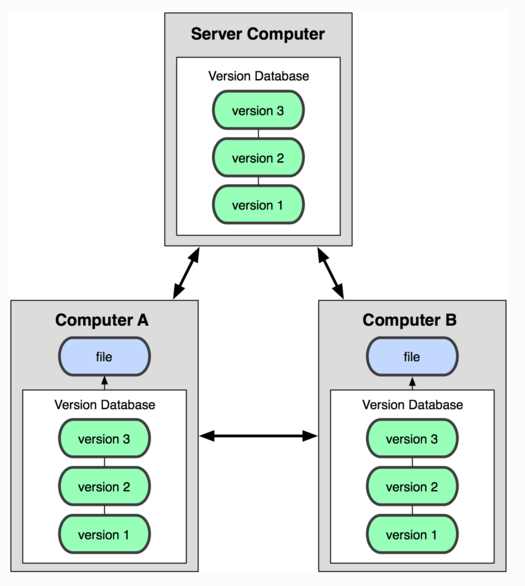
\includegraphics[scale=0.5]{pictures/vcs.png}
\end{center}
\caption{Sistemi za kontrolu verzija.}
\label{fig:storage}
\end{figure}

Postoji više sistema za kontrolu verzija, neki od najpoznatijih su:
\begin{itemize}
\item GitHub
\item GitLab
\item CVS
\item BitBucket
\item AWS
\end{itemize}  

U nastavku će detaljnije biti objašnjeno korišćenje sistema $GitHub$.

\subsection{GitHub}

$GitHub$ je nastao $2005.$ godine i predstavlja jedan od najpopularnijih sistema za kontrolu verzija. U nastavku biće objašnjene neke od osnovnih naredbi kroz korišćenje terminala. Postojanje GitHub naloga se podrazumeva. Za podešavanje okruženja na $Windows$-u koristiti: https://gitforwindows.org/. Za podešavanje na $Linuxu$ korisiti $sudo\ apt-get\ install\ git$.\\\\

\begin{figure}[h!]
\begin{center}
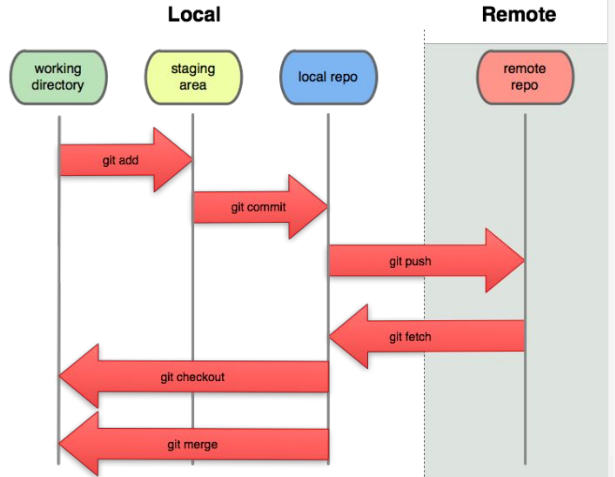
\includegraphics[scale=0.5]{pictures/git_diag.png}
\end{center}
\caption{Dijagram.}
\label{fig:storage}
\end{figure}

\subsubsection{Osnovne Git naredbe}
Nakon što je kreiran nalog na $GitHub$-u neophodno je izvršiti povezivanje. Postoji nekoliko načina povezivanja u zavisnosti od platforme. Autor savetuje korišćenje terminala.

Kucanjem komande $git$ u terminalu izlazi spisak najčešće korišćenih komandi:
\begin{verbatim}
$ git 
\end{verbatim}

Neke od njih su:
\begin{itemize}
\item clone
\item init
\item add
\item mv
\item reset
\item rm
\item commit 
\item push
\item merge
\end{itemize}

Za započinjanje radnog direktorijuma koriste se komande $git\ clone$ ili $git\ init$. Sa $git\ clone$ vršimo kopiranje postojećeg direktorijuma u lokal. Sa $git\ init$ kreiramo prazan $Git$ repozitorijum. Za više, otkucati $git\ help\ tutorial$.

\begin{verbatim}
$git clone linkkarepozitorijumu
$git init nazivrepozitorijuma
\end{verbatim}

Za rad na trenutnim promenama, koriste se komande $add$, $mv$, $rm$ i $reset$. Prva komanda dodaje sadržaj fajla (ili više njih uz pojedinačno navođenje ili svih opciju --all). Druga komanda služi za premeštanje fajlova ili direktorijuma. Treća komanda vrši brisanje. Za više, otkucati $git\ help\ everyday$. 
\begin{verbatim}
$git add nazivfajla
$git add nazivfajla1 nazivfajla2
$git add --all
$git mv nazivfajla
$git rm nazivfajla
\end{verbatim}


Da bi se videle promene i trenutno stanje koristiti komandu $status$. Za više, otkucati $git\ help\ revisions$.
\begin{verbatim}
$git status
\end{verbatim}

Da bi se sačuvale promene učinjene nad repozitorijumom koristiti komandu $commit$. 
\begin{verbatim}
$git commit 
\end{verbatim}
Sa $-m$ piše se poruka kojom treba opisati ukratko šta je promenjeno, na primer ako je dodat neki modul. Poruka je najčešće oblika $"$učinjena akcija-nad kojim objektom$"$
\begin{verbatim}
$git commit -m "Added module X."
\end{verbatim}

Rad na projektu na kojem učestvuje više ljudi zahteva korišćenje grana. Glavna grana na kojoj se nalazi projekat naziva se $master$ granom. Ostale kreirane grane bi trebalo da predstavljaju rad pojedinačnih članova. Nakon što kod prođe reviziju, komandom $merge$ vrši se spajanje grane sa glavnom (ili spajanje različitih grana). Komandom $branch$ mogu se izlistati, kreirati ili brisati grane u zavisnosti od dodatnih opcija. Sa $checkout$ vrši se proemna grane. Praćenje promena između $commit$-ova vrši se komandom $diff$. \\\\
Napomena: prilikom navođenja komandi neophodno je da budu oblika $git\ nazivkomande\ opcije$, a onda eventualno fajl ili fajlovi (direktorijum ili direktorijumi).\\\\
Da bismo promene prebacili sa lokala na server, neophodno je da iskoristimo komandu $push$. Nakon što je otkucamo u terminalu će nam se tražiti da unesemo korisničko ime i lozinku za nalog na $GitHub$-u.Prilikom saradnje sa drugima, osim gore navedenih komandi, korisne su i $fetch$ koja skida određeni repozitorijum, $pull$ koja povlači izmene ili direktorijum. Za više, otkucati $git\ help\ workflows$. 

\begin{figure}[h!]
\begin{center}
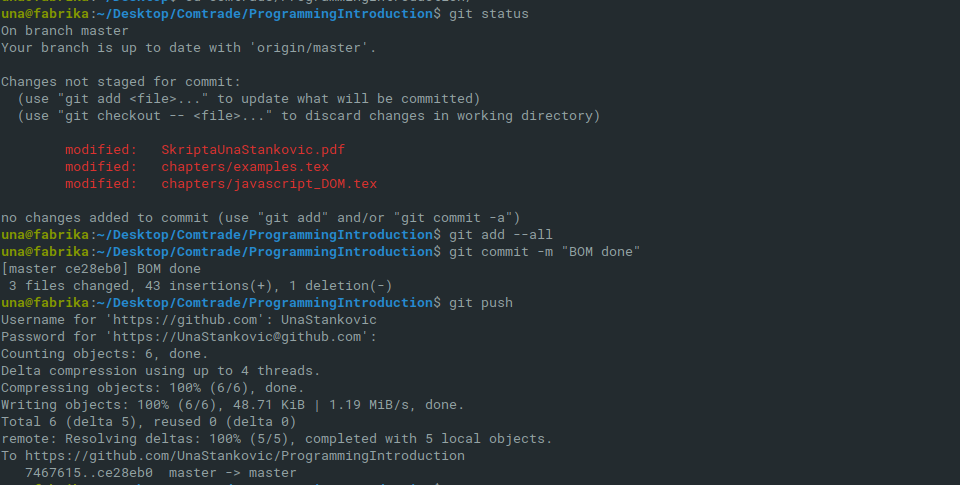
\includegraphics[scale=0.5]{pictures/git.png}
\end{center}
\caption{Primer prebacivanja promena.}
\label{fig:storage}
\end{figure}

\subsubsection{README}
README fajl predstavlja veoma važan deo svakog $git$ repozitorijuma. On treba da sadrži ukratko opisan projekat, način pokretanja projekta, tehnologije korišćene pri razvoju, imena svih učesnika u razvoju projekta, verzije i ostale relevantne informacije. Primer $README$ fajla:

\begin{lstlisting}[backgroundcolor = \color{lightgray}, breaklines=true]
FindingRedundantTestExamples
This project is a part of our Master Studies' course of Software Verification. The main idea is to explore, experiment and try to develop a methodology of discovering and removing redundant test examples. This project is done in collaboration with Mirko Ivanovic and Milos Petrovic who also attend the course during summer semester of 2018.

In the .tex file there are sections which represent out train of thoughts. There we have presented various ideas, experiments done and tools used in a process. The whole text is written in Serbian.

usage of test runs
Requirements:
    - clang-format-6.0
    - python (compatible with python3)
    - numpy package

Usage:
    - run python script redundant_test_runs/redundant_tests.py
	- run example:
        cd redundant_test_runs
        python3 redundant_tests.py
        c
        examples/01
		
Available examples:
    examples/01
    examples/02
    examples/03
    examples/04
usage of custom unit testing framework
Requirements:
    - clang-format-6.0
    - python (compatible with both python2.7 and python3)
    - numpy package

Setup:
    - cd redundant_unit_test_framework
    - Run ./setup.sh (compiles custom unit testing framework)

Usage:
    - Input
        python redundant_tests.py examples/01 
    - Output
        Redundant tests: 
        tst_03.test_deljenje2
		
    - Input (general usage)
        python redundant_tests.py {path to a test project} 
    - Output
        Redundant tests:
        {list of redundant tests}
        
Available examples:
    - examples/01
    - examples/02
    - examples/03_false_positives
    - examples/04
    - examples/05_loop
\end{lstlisting}

\subsubsection{.gitignore}
Često pri radu na projektu generiše se dosta fajlova koji su privremeni ili za koje ne želimo da budu podignuti u repozitorijum. Da bismo sprečili podizanje ovakvih fajlova koristimo .gitignore fajl. Naime, u fajlu sa ovim nazivom u novoj liniji navodimo ekstenzije fajlova koje želimo da ignorišemo:

\begin{lstlisting}[backgroundcolor = \color{lightgray}, breaklines=true]
*.pyc
*.c~
*.py~
*.log
*.aux
*.out
*.toc
*.synctex.gz
*.bbl
*.blg
*.o
*.exe 
\end{lstlisting}

\subparagraph{Zadaci- Sistemi za kontrolu verzija}

\begin{primer}
Klonirati neki od postojećih git direktorijuma i istražiti šta se sve nalazi u njemu.
\end{primer}

\begin{primer}
Kreirati projekat sa nazivom zdravstvena stanica. Dodavati komponente stranice redom (html, css, JS i ostale fajlove). Svaka završena celina treba da predstavlja jedan commit. Svaki commit treba da sadrži adekvatan komentar.
\end{primer}

